\chapter{Analyse \& analyse numérique pour le système de Stokes}

Ce chapitre est dédié à la compréhension de la physique, de l'analyse puis du développement numérique par les volumes finis des problèmes d'écoulement fluides visqueux. On travaillera en particulier sur le problème de Stokes. La rédaction de l'analyse de cette partie est calquée sur le cours de Yannick Privat et Pascal Frey donné dans le cadre du master de modélisation de Sorbonne-Université lors de l'année 2020 / 2021. Les documents sont disponibles sur la \href{https://www.ljll.math.upmc.fr/frey/nm491.html}{page du cours} : https://www.ljll.math.upmc.fr/frey/nm491.html. La partie numérique se fait à l'aide de la méthode des volumes finis sur maillage marker \& cells. 

\section{Modélisation des fluides visqueux}

Un fluide est d'abord décrit par la place qu'il occupe dans $\mathbb{R}^d$, on choisira un ouvert connexe borné et régulier, lipschitzien au moins, comme domaine fluide, noté $\Omega$.

L'état d'un fluide formulé en variables eulériennes est décrit par un champ de vitesses $\mathbf{v} : \Omega \rightarrow \mathbb{R}^d$ et d'une ou plusieurs grandeurs scalaires : la pression $p : \Omega \rightarrow \mathbb{R}$ toujours, et parfois d'autres, selon la phénoméologie du problème. Par exemple, des variables thermodynamiques peuvent être considérées : température, entropie, etc. Dans ce cas le système de Stokes se complète par la définition d'une entropie et le système devient celui de Stokes augmenté de la conservation de cette entropie. Ce mémoire se limite à la description en vitesses et pression. 

Les fluides sont caractérisés par une masse volumique $\rho : \Omega \rightarrow \mathbb{R}$, exprimée en $kg.m^{-3}$. Dans la suite, nous la considérerons constante. Dans le cas du fluide visqueux, on dispose également d'une viscosité dynamique $\mu : \Omega \rightarrow \mathbb{R}$, que nous prendrons constante également.

La dynamique d'un fluide visqueux soumis à une densité de force $\mathbf{f}$ est décrite par le système de Navier-Stokes
\begin{equation*}
    \partial_t \rho + \nabla \cdot (\rho \mathbf{v}) = g
\end{equation*}
est l'équation de continuité, qui s'interprète comme la conservation de la masse et 
\begin{equation*} \tag{N-S}
    \partial_t (\rho \mathbf{v}) + (\mathbf{v} \cdot \nabla) \mathbf{v} + \nabla p - \mu \Delta \mathbf{v} = \rho \mathbf{f}
\end{equation*}
décrit la conservation des moments.

\section{Approximation de Stokes : les faibles nombres de Reynolds}

Supposons que $\rho = 1$ et $\mu = 1$. Comme expliqué dans \cite{jpc}, l'équation de Navier-Stokes pour l'écoulement d'un fluide newtonien homogène et incompressible s'écrit, après adimensionnement par $\rho V_0^2$ : 
\begin{align*}
    \nabla \cdot \mathbf{v} = 0 \\
    \partial_t v(t; \mathbf{x}) + \left( \mathbf{v} \cdot \nabla \right) \mathbf{v} - \frac{1}{Re} \nabla^2 \mathbf{V} + \nabla p = 0
\end{align*}
Si on fait tendre le nombre de Reynolds vers 0 alors on trouve à la limite l'équation de Laplace $\nabla^2 \mathbf{v} = 0$, qui est inconsistante avec la condition d'incompressibilité. Par exemple, l'écoulement laminaire incompressible stationnaire entre deux plans
\begin{align*}
    \frac{d^2 u}{dy^2}(y) = 0 \\
    u(0) = 0 \\
    u(1) = 0
\end{align*}
donne une solution $u$ identiquement nulle. Ceci résulte d'un mauvais choix pour l'adimensionnement de la pression : l'adimensionnement se fait via le termes d'inertie, négligé dans ce second système, or il est nécessaire de considérer plutôt les forces visqueuses par unité de surface, l'adimensionnement se faisant donc par le facteur $\frac{\mu V_0}{H}$, $H$ étant la hauteur séparant les deux plans.

\paragraph{L'équation de Stokes stationnaire avec conditions de Dirichlet homogène} Soit un fluide occupant une région $\Omega$ ouverte, connexe, régulière et bornée de $\mathbb{R}^d$ avec $d \in \llbracket 1, 3\rrbracket$. L'équation de Stokes stationnaire en l'absence de création de masse s'écrit
\begin{align*}
    \nabla \cdot \mathbf{v} = 0 & \hspace{15pt} \Omega \\
    -\mu \Delta \mathbf{v} + \nabla p = \rho \mathbf{f} & \hspace{15pt} \Omega \\
    u = 0 & \hspace{15pt} \partial \Omega
\end{align*}
où $f : \Omega \rightarrow \mathbb{R}^d$. La première est l'équation de conservation de la masse et la seconde l'équation de conservation du moment. Dans le cas où on aurait une fonction source de masse $g : \Omega \rightarrow \mathbb{R}$, il faudrait observer une condition de compatibilité supplémentaire. Du fait que $$ \int_\Omega \nabla \cdot \mathbf{v} dx = \int_K g(x) dx $$ le théorème de la divergence donnant l'égalité $$ \int_\Omega (\nabla \cdot \mathbf{v})(x) dx = \int_{\partial \Omega} (\mathbf{v} \cdot \mathbf{n})(\gamma(x)) d\gamma(x) $$ on doit imposer à $g$ la contrainte $$ \int_\Omega g(x) dx = 0 $$

\paragraph{Définition d'une solution classique} Un couple $\begin{pmatrix} \mathbf{v} \\ p \end{pmatrix}$ est une solution classique du problème de Stokes stationnaire si, et seulement si ce couple appartient à $\left( \mathcal{C}^2(\Omega) \cap \mathcal{C}^0(\bar{\Omega})\right) \times \mathcal{C}^1(\Omega)$

Une solution classique, lorsqu'elle existe, n'est pas unique. En effet, si $\begin{pmatrix} \mathbf{v} \\ p \end{pmatrix}$ est solution, alors pour toute constante $c \in \mathbb{R}$, le couple $\begin{pmatrix} \mathbf{v} \\ p+c \end{pmatrix}$ en est une également. Dans le cas d'une solution classique, il est suffisant de fixer la valeur de $p$ en un point.

\paragraph{Exemples de solutions classiques} L'ouvrage \cite{jpc}, chapitre 4 section 2 propose des exemples de solutions exactes pour le problème de Stokes en une dimension.

Par exemple, l'écoulement de Poiseuille plan. Il décrit l'écoulement généré par un gradient horizontal de pression sur un fluide confiné entre deux plans parallèles aux altitudes $y=0$ et $y=H$. L'écoulement est supposé être laminaire, incompressible, stationnaire et établi. L'hypothèse de laminarité signifique que l'écoulement est parallèle aux parois solides, donc le problème de Stokes se réduit à
\begin{equation*} \tag{P}
    \mu \partial^2_{y,y} u = \frac{dp}{dy} 
\end{equation*}
Cette équation est une E.D.O d'ordre 2, dont les constantes d'intégrations sont déterminées par les vitesses en $0$ et $H$. Si le gradient de pression dans le sens de l'écoulement est noté $\Delta_x p$, constant, alors $$ u : y \mapsto -\frac{H^2}{8\mu} \Delta_x p \left( 4\frac{y}{H} - 4\frac{y^2}{H^2} \right) $$

\begin{figure}[htp]
    \centering
    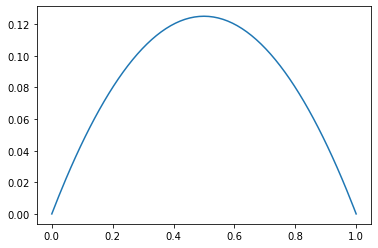
\includegraphics[width=7.5cm]{Images/stokes/solutions/poiseuillePlan.png}
    \caption{En absisse : l'altitude $y$, en ordonnée, la norme de la vitesse horizontale.}
\end{figure}

En deux dimensions, on utilisera une variante du triplet de Taylor-Green adapté au système de Stokes. Dans sa version stationnaire, ces fonctions sont données par

\begin{align*}
    u : x, y \mapsto & sin(x) cos(y) \\
    v : x, y \mapsto & -cos(x) sin(y) \\
    p \equiv &  C \in \mathbb{R}
\end{align*}
où $u,v$ sont les deux composantes du vecteur $\mathbf{v}$. Ce triplet vérifie la contrainte $\nabla \cdot \mathbf{v} = 0$ en tout point de $\Omega$. On présente le champ de vecteur pour un tourbillon

\begin{figure}[htp]
    \centering
    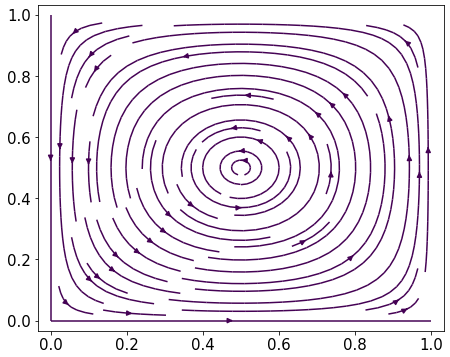
\includegraphics[width=7.5cm]{Images/stokes/solutions/taylorGreenStream.png}
    \caption{Courbes intégrales du champ $\mathbf{v}$ pour un tourbillon}
\end{figure}

\paragraph{Cadre fonctionnel pour Stokes stationnaire et conditions homogènes en vitesse} Soit $\mathcal{D}(\Omega)^d$ l'espace des fonctions $\mathcal{C}^{\infty}_c(\Omega)^d$ l'espace des fonctions tests. On note $V := H^1_0(\Omega)^d$ muni de sa structure hilbertienne. Notons enfin $Q := \{ L^2_0(\Omega) := \{ q \in L^2(\Omega), \int_\Omega q(x) dx = 0 \}$.

Soit $f \in L^2(\Omega)^d$, soient $\mathbf{v}$, $\mathbf{w} \in V$, multiplions l'équation de conservation des moments et intégrons sur $\Omega$ : $$ -\mu \int_{\Omega} \Delta \mathbf{v} \cdot \mathbf{w} dx + \int_\Omega \nabla p \cdot \mathbf{w} dx = \rho \int_\Omega \mathbf{f} \cdot \mathbf{w} dx $$ La première intégrale vérifie les hypothèses du théorème de la divergence : $$ \int_\Omega \Delta \mathbf{v} \cdot \mathbf{w} dx = \int_\Omega \nabla \mathbf{v} : \nabla \mathbf{w} dx - \int_{\partial \Omega} \partial_{\mathbf{n}} \mathbf{v} \cdot \mathbf{w} d\gamma(x) $$ avec le second terme du membre de droite nul par hypothèse. L'intégrale portant sur le gradient de pression s'intègre également par parties, soit $$ \int_\Omega \nabla p \cdot \mathbf{w} dx = - \int_\Omega p \nabla \cdot \mathbf{w} dx $$ si bien qu'on trouve pour l'équation du moment $$ \mu \int_\Omega \nabla \mathbf{v} : \mathbf{w} dx - \int_\Omega p \nabla \cdot \mathbf{w} = \int_\Omega \mathbf{f} \cdot \mathbf{w} dx $$

L'équation de continuité se traite de la même manière. Choisissons $q \in Q$ et en intégrons sur le domaine $\Omega$, alors une intégration par parties donne l'expression $$ \int_\Omega q \nabla \cdot \mathbf{v} dx = 0 $$

Il est possible, grâce à l'identification de $L^2(\Omega)$ avec son dual topologique via le produit scalaire et des propriétés des injections $H^1_0(\Omega)^d \hookrightarrow L^2(\Omega) \equiv L^2(\Omega) \hookrightarrow H^{-1}(\Omega)^d$ de considérer des fonctions $\mathbf{f}$ dans $H^{-1}(\Omega)^d$. Dans ce cas le terme $\int_\Omega \mathbf{f} \mathbf{w} dx$ se lit comme le crochet de dualité $< \mathbf{f}, \mathbf{w} >_{H^{-1}, H^1_0}$.

On introduit les deux formes $ a := V \times V \rightarrow \mathbb{R} $ et $ b: V \times Q \rightarrow \mathbb{R} $, définies par les expressions $$ a(\mathbf{v}, \mathbf{w}) := \int_\Omega \nabla \mathbf{v} : \nabla \mathbf{w} dx $$ et $$ b(\mathbf{w}, q) := -\int_\Omega q \nabla \cdot \mathbf{w} dx $$ On introduit enfin $f : V \rightarrow \mathbb{R}$, $$ f(\mathbf{w}) := \int_\Omega \mathbf{f} \cdot \mathbf{w} dx $$ Avec ces notations, la formulation variationnelle du problème s'écrit, avec $\mathbf{f} \in H^{-1}(\Omega)^d$,

Trouver $\mathbf{v} \in V, p \in Q$
\begin{align*}
     a(\mathbf{v}, \mathbf{w}) + b(\mathbf{w}, p) = f(v) \hspace{15pt} \forall \mathbf{w} \in V \\
     b(\mathbf{v}, q) = 0 \hspace{15pt} \forall q \in Q
\end{align*}

On a la proposition suivante
\begin{proposition}
    Si $f$ est $L^2(\Omega)$ alors une solution $(\mathbf{v}, p)$ de la formulation variationnelle est solution du problème de Stokes stationnaire.
\end{proposition}

La preuve se fait par approximations sur $\mathbf{w}$. Pour tout $\mathbf{w} \in \mathcal{D}(\Omega)$, on a, au sens des distributions $$ < - \Delta \mathbf{v} + \nabla p, \mathbf{w} >_{\mathcal{D}', \mathcal{D}} = \int_\Omega \mathbf{f} \mathbf{w} dx $$ Par densité, pour $\mathbf{w}$ dans $V$, on choisit une approximation $\left(\mathbf{w}_n\right)_n$ de $\mathbf{w}$ pour la norme hilbertienne sur $V$ et on montre alors que $$ - \Delta \mathbf{v} + \nabla p = \mathbf{f} $$ toujours au sens des distributions. Il en va de même pour l'équation de continuité. De plus, les conditions aux limites sont imposées par définition de $V := H^1_0(\Omega)^d$. 

\paragraph{Formulation comme point selle d'un lagrangien} En guise de remarque préliminaire, on note que $Q$ est un espace réflexif, donc que $Q = Q''$. On introduit alors les opérateurs $$ A : V \rightarrow V' \hspace{15pt} <A\mathbf{v}, \mathbf{w}>_{V', V} = a(\mathbf{v}, \mathbf{w}) $$ et $$ B : V \rightarrow Q' \hspace{15pt} <B\mathbf{w}, q>_{Q', Q} $$ On admet alors que trouver une solution au problème variationnel est équivalent à
trouver $\mathbf{v} \in V$, $p \in Q$ tel que
\begin{align*}
    A\mathbf{v} + B^T p = 0 \\
    B\mathbf{v} = 0
\end{align*}

On introduit donc le noyau de l'opérateur $B$ : $$ ker(B) := \{ \mathbf{v} \in V, \forall q \in Q, b(\mathbf{v}, q) = 0 \} $$ et on introduit le projecteur $$ \pi_A : ker(B) \rightarrow ker(B)' $$ défini par $ < \pi_A \mathbf{v}, \mathbf{w}>_{V', V} = < A\mathbf{v}, \mathbf{w} >_{V', V} $ pour tout $\mathbf{v} \in ker(B)$.

On cite le théorème

\begin{theoreme}
    Avec les notations précédentes, sous les hypothèses suivantes
    \begin{itemize}
        \item $V$ est réflexif,
        \item $Q$ est réflexif,
        \item $\mathbf{f}$ est un élément de $V'$,
        \item $a \in \mathcal{L}(V \times V ; \mathbb{R})$ est bilinéaire,
        \item $b \in \mathcal{L}(V \times Q ; \mathbb{R})$ est bilinéaire,
    \end{itemize}
    alors il existe une unique solution au problème variationnel si, et seulement si,
    \begin{equation*}
        \left\{
        \begin{array}{l}
            \exists \alpha > 0 : \inf_{\mathbf{v} \in ker(B)} \sup_{\mathbf{w} \in ker(B)} \frac{a(\mathbf{v}, \mathbf{w})}{\| \mathbf{v} \| \| \mathbf{w} \|} \geqslant \alpha \\
            \forall \mathbf{w} \in ker(B), \left( \forall \mathbf{v} \in ker(B), a(\mathbf{v}, \mathbf{w} \right) \Rightarrow \mathbf{w} = 0
        \end{array}
        \right.
    \end{equation*}
    et si
    \begin{equation*}
        \exists \beta > 0 : \inf_{q\in Q} \sup_{\mathbf{v}\in V} \frac{b(\mathbf{v}, q)}{\|\mathbf{v}\|_V \|q\|_Q} \geqslant \beta
    \end{equation*}
    De plus, on a les estimations a priori
    \begin{align*}
        \|\mathbf{v}\|_V & \leqslant \alpha^{-1} \|f\|_{V'} \\
        \|p\|_Q & \leqslant \beta^{-1} \left( 1 + \frac{\|a\|}{\alpha} \right) \| f \|_{V'}
    \end{align*}
\end{theoreme}

Ce théorème, issu du cours de messieurs Frey et Privat, trouve en partie sa démonstration dans \cite{bernardi}, chapitre 1.

\begin{definition}
    Soient $V, Q$ deux espaces de Banach réflexifs, soit $\mathcal{L}(V\times Q ; \mathbb{R})$, alors un couple $(\mathbf{v}, p)$ est un point selle du lagrangien $\mathcal{L}$ si $$ \forall (\mathbf{w}, q) : \mathcal{L}(\mathbf{v}, q) \leqslant \mathcal{L}(\mathbf{v}, p) \leqslant \mathcal{L}(\mathbf{w}, p) $$
\end{definition}

Un point selle se caractérise par la proposition

\begin{proposition}
    Un couple $(\mathbf{v}, p)$ est un point selle pour $\mathcal{L}$ si, et seulement si,
    $$ \inf_{\mathbf{w} \in V} \sup_{q\in Q} \mathcal{L}(\mathbf{w}, q) = \sup_{q \in Q} \mathcal{L}(\mathbf{v}, q) = \inf_{\mathbf{w}\in V} \mathcal{L}(\mathbf{w}, p) = \sup_{q \in Q} \inf_{\mathbf{w} \in V} \mathcal{L}(\mathbf{w}, q) $$
\end{proposition}

Dans le cas où $a$ est symétrique et définie positive, on dispose du résultat
\begin{proposition}
    Si $a$ est symétrique et définie positive alors $(\mathbf{v}, p)$ est solution du problème variationnel si, et seulement si, ce couple est point selle du lagrangien $$ \mathcal{L}(\mathbf{w}, q) := \frac{1}{2} a(\mathbf{w}, \mathbf{w}) + b(\mathbf{w}, q) - f(\mathbf{w}) $$
\end{proposition}
qui permet de montrer que dès lors que $a$ est symétrique et définie positive, si les conditions $\inf \sup$ sont toutes deux réalisées, alors
\begin{itemize}
    \item le problème variationnel admet une unique solution,
    \item cette solution est l'unique point selle de la forme $\mathcal{L}$ telle que définie dans la proposition précédente,
    \item la solution vérifie la caractérisation d'un point selle.
\end{itemize}

On peut enfin conclure cette section par le résultat 

\begin{theoreme}
    Le problème de Stokes stationnaire avec conditions aux limites de Dirichlet homogène en vitesse admet une unique solution et existe un réel strictement positif $c > 0$ tel que, quel que soit $\mathbf{f} \in H^{-1}(\Omega)^d$ $$ \| \mathbf{v} \|_{H^1(\Omega)^d} + \|p \|_{L^2(\Omega)} \leqslant c \| f \|_{H^{-1}} $$
\end{theoreme}

La preuve se fait grâce aux développements précédents avec $B := \nabla \cdot : H^1_0(\Omega)^d \rightarrow L^2_0(\Omega)$ ; $ker(B) := V_0 = \{ \mathbf{w} \in H^1_0(\Omega)^d, \nabla \cdot \mathbf{w} = 0 \}$

Numériquement, l'imposition de la condition de Dirichlet en un point permettant de fixer la constante pour $p$ ne fait pas sens pour une fonction $L^2(\Omega)$ en général. On discrétisera donc la moyenne de $p$, dont la valeur est notée $M$ : $$ \bar{p} = M \Longleftrightarrow \frac{\Delta y \Delta x}{|\Omega|} \sum p_{j,i} = M $$ dans le cas d'un maillage rectangulaire uniforme.

\paragraph{Autre formulation du problème de Stokes} Le problème de Stokes peut également se formuler à l'aide du tenseur des contraintes, ou tenseur de Cauchy du fluide. On le note $\sigma := -\mu\left( \nabla \mathbf{v} + \mathbf{v}^T \right) - p \text{Id}_{\mathbb{R}^d}$. Dans ce cas le système de Stokes s'écrit comme un système de lois de conservations adapté à une discrétisation par méthode de volumes finis
\begin{align*}
    \nabla \cdot \mathbf{v} = 0 \\
    \nabla \sigma(\mathbf{v}, p) = \mathbf{f}
\end{align*}


\section{Maillage Marker \& Cell}

\paragraph{Le maillage M.A.C} Le maillage markers \& cells est une grille décalée en vitesse et en pression. Par convention, on fixe les noeuds de pression aux bords. Un exemple en une dimension avec noeuds de pression aux bords

\begin{figure}[htp]
    \centering
    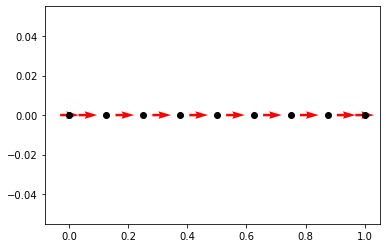
\includegraphics[height=3cm, width=7.5cm]{Images/preliminaires/maillages/MAC 1D.png}
    \caption{En noir, les points de pression, au milieu des flèches rouge les points de vitesse.}
\end{figure}

\newpage

En deux dimensions, la cavité $[0,1]\times[0,1]$ discrétisée par un maillage rectangulaire de $8 \times 8$ volumes M.A.C est sur la figure suivante.

\begin{figure}[htp]
    \centering
    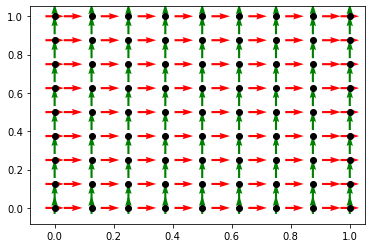
\includegraphics{Images/preliminaires/maillages/MAC 2D.png}
    \caption{En noir, les points de pression, au milieu des flèches vertes, les points de composante verticale de la vitesse et au milieu des flèches rouge les points de composante horizontale de la vitesse.}
\end{figure}

On dispose de $(n_y+1)(n_x+2)$ points de composante horizontale de vitesse, $(n_y+2)(n_x+1)$ points de composante verticale de vitesse et $(n_y+1)(n_x+1)$ points de pression, leur somme étant le nombre d'inconnues. On les numérote par type et dans l'ordre lexicographique, lisant de gauche à droite, de bas vers le haut. Le vecteur d'état inconnues est posé comme étant $$ X := \begin{pmatrix} U_h \\ V_h \\ P_h \end{pmatrix} $$ Dans la prochaine section, on développe trois codes : deux pour le Laplacien de Dirichlet sur les sous-maillages de vitesse et un Laplacien de Neumann pour le sous-maillage de pression.

\paragraph{Laplacien de Dirichlet sur le maillage de $U_h$} On reprend l'étude du Laplacien avec conditions de Dirichlet sur les bords. Si le schéma à l'intérieur s'écrit de la même manière que celle développée dans le premier chapitre du mémoire, un fait change : les inconnues $U_{h,0,i}$ et $U_{h,n_y,i}$ vérifient directement la condition de Dirichlet, on n'y discrétise pas le Laplacien, en revanche on écrit le Laplacien discret sur les colonnes $U_{h,j,1}$ et $U_{h,j,n_x}$. Les relations sur les colonnes ne font intervenir que quatre inconnues et imposent une modification du second membre. On présente le code apaté à ce problème

\begin{minted}{python}
from matplotlib import pyplot
import numpy
from numpy import cos, pi, sin
from scipy import sparse
from scipy.sparse.linalg import gmres, splu

# SETUP
u_func  = lambda x, y : sin(x) * cos(y)
Su_func = lambda x, y : 2 * u_func(x, y)

# DISCRETISATION SPATIALE
## Horizontale
xi = 0.
xf = 2*pi
nx_ = numpy.array([4, 8, 16, 32, 64, 128, 512, 1024])
dx_ = (xf-xi)/nx_

## Verticale
yi = 0.
yf = 2*pi

# INITIALISATION
err = numpy.zeros(nx_.shape)

# ANALYSE DU SCHEMA
for k, nx in enumerate(nx_):
    
    # Discrétisation spatiale
    dx = dx_[k]
    ny = nx
    print("> Maillage {}x{}".format(ny, nx))
    dy = (yf-yi)/ny
    Ox = numpy.linspace(xi+dx/2, xf-dx/2, nx)
    Ox = numpy.concatenate([[xi], Ox, [xf]], axis=0)
    Oy = numpy.linspace(yi, yf, ny+1)
    X, Y = numpy.meshgrid(Ox, Oy)
    
    # Construction de l'opérateur discret
    N = 5*(ny-1)*nx + 2*(ny-1) + 2*(nx+2)
    lignes   = numpy.zeros(N)
    colonnes = numpy.zeros(N)
    donnees  = numpy.zeros(N)
    
    b = (dy*dx) * Su_func(X, Y)
    b[0, :] = u_func(Ox, yi)
    b[-1,:] = u_func(Ox, yf)
    b[:, 0] = u_func(xi, Oy)
    b[:,-1] = u_func(xf, Oy)

    compteur = 0
    for j in range(ny+1):
        for i in range(nx+2):
                
            if i == 0 or i == nx+1 or j == 0 or j == ny:
                lignes[compteur]   = j * (nx+2) + i
                colonnes[compteur] = j * (nx+2) + i
                donnees[compteur]  = 1
                compteur += 1
   
            elif i == 1:
                lignes[compteur : compteur+5] = j * (nx+2) + i
                colonnes[compteur]   = j * (nx+2) + i
                colonnes[compteur+1] = j * (nx+2) + i - 1
                colonnes[compteur+2] = j * (nx+2) + i + 1
                colonnes[compteur+3] = (j-1) * (nx+2) + i
                colonnes[compteur+4] = (j+1) * (nx+2) + i
                donnees[compteur]    = 3*(dy/dx) + 2*(dx/dy)
                donnees[compteur+1]  = -2*dy/dx
                donnees[compteur+2]  = -dy/dx
                donnees[compteur+3]  = -dx/dy
                donnees[compteur+4]  = -dx/dy
                compteur += 5
            
            elif i == nx:
                lignes[compteur : compteur+5] = j * (nx+2) + i
                colonnes[compteur]   = j * (nx+2) + i
                colonnes[compteur+1] = j * (nx+2) + i - 1
                colonnes[compteur+2] = j * (nx+2) + i + 1
                colonnes[compteur+3] = (j-1) * (nx+2) + i
                colonnes[compteur+4] = (j+1) * (nx+2) + i
                donnees[compteur]    = 3*(dy/dx) + 2*(dx/dy)
                donnees[compteur+1]  = -dy/dx
                donnees[compteur+2]  = -2*dy/dx
                donnees[compteur+3]  = -dx/dy
                donnees[compteur+4]  = -dx/dy
                compteur += 5

            else:
                lignes[compteur : compteur+5] = j * (nx+2) + i
                colonnes[compteur]   = j * (nx+2) + i
                colonnes[compteur+1] = j * (nx+2) + i - 1
                colonnes[compteur+2] = j * (nx+2) + i + 1
                colonnes[compteur+3] = (j-1) * (nx+2) + i
                colonnes[compteur+4] = (j+1) * (nx+2) + i
                donnees[compteur]    = 2 * (dy/dx + dx/dy)
                donnees[compteur+1]  = -dy/dx
                donnees[compteur+2]  = -dy/dx
                donnees[compteur+3]  = -dx/dy
                donnees[compteur+4]  = -dx/dy
                compteur += 5

    A = sparse.coo_matrix((donnees, (lignes, colonnes)), shape=((ny+1)*(nx+2), (ny+1)*(nx+2))).tocsc()
    Ma = sparse.linalg.LinearOperator(((ny+1)*(nx+2), (ny+1)*(nx+2)), splu(A).solve)
    
    U = gmres(A, b.flatten(), M=Ma)[0].reshape(ny+1, nx+2)
    
    u = u_func(X, Y)
    err[k] = numpy.sqrt(dy*dx) * numpy.linalg.norm(U-u, ord=2)

# FIGURES
pyplot.figure()
pyplot.loglog(nx_, err, 'x-', label=r"$||U-u||_{L^2}$")
pyplot.loglog(nx_, dx_, '--', label=r"$\Delta x$")
pyplot.loglog(nx_, dx_**2, '--', label=r"$\Delta x^2$")
pyplot.legend()
pyplot.show()

pyplot.figure()
pyplot.imshow(numpy.abs(U-u))
pyplot.colorbar()
pyplot.show()
\end{minted}
avec un champ d'erreurs et la courbe d'erreur de consistance en norme $L^2(\Omega)$

\begin{figure}[htp]
    \centering
    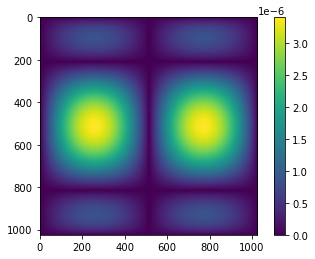
\includegraphics[width=7.5cm]{Images/stokes/Laplace Dirichlet 2D (U)/erreur.png}
    \caption{Champ d'erreurs pour le Laplacien sur $\mathcal{T}^U$}
\end{figure}

\begin{figure}[htp]
    \centering
    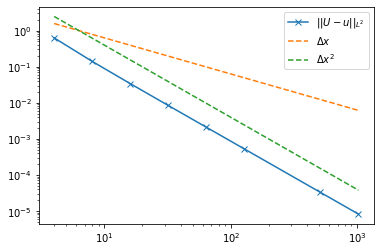
\includegraphics[width=7.5cm]{Images/stokes/Laplace Dirichlet 2D (U)/analyse.png}
    \caption{Analyse de la norme $L^2(\Omega)$ pour le Laplacien sur $\mathcal{T}^U$}
\end{figure}

\paragraph{Laplacien de Dirichlet sur le maillage de $V_h$} De même pour le laplacien sur $\mathcal{T}^V$ : le schéma au centre est le même, le schéma aux bords verticaux est réduit à $V_{h,j,0} = V^D(x_0, y_{j+1/2})$, $V_{h,j,n_x} = V^D(x_{n_x}, y_{j+1/2})$ et les lignes $j=1$ et $j=n_y$ font appel à un noeud fantôme et donc à une substitution.

\begin{minted}{python}
from matplotlib import pyplot
import numpy
from numpy import cos, pi, sin
from scipy import sparse
from scipy.sparse.linalg import gmres, splu

# SETUP
u_func  = lambda x, y : sin(x) * cos(y)
Su_func = lambda x, y : 2*u_func(x, y)

# DISCRETISATION SPATIALE
## Horizontale
xi = 0.
xf = 2*pi
nx_ = numpy.array([4, 8, 16, 32, 64, 128, 256, 512, 1024])
dx_ = (xf-xi)/nx_

## Verticale
yi = 0.
yf = 2*pi

# INITIALISATION
err = numpy.zeros(nx_.shape)

# ANALYSE DU SCHEMA
for k, nx in enumerate(nx_):
    
    # Discrétisation spatiale
    dx = dx_[k]
    ny = nx
    print("> Maillage {}x{}".format(ny, nx))
    dy = (yf-yi)/ny
    Ox = numpy.linspace(xi, xf, nx+1)
    Oy = numpy.linspace(yi+dy/2, yf-dy/2, ny)
    Oy = numpy.concatenate([[yi], Oy, [yf]], axis=0)
    X, Y = numpy.meshgrid(Ox, Oy)
    
    # Construction de l'opérateur discret
    N = 5*ny*(nx-1) + 2*(ny+2) + 2*(nx-1)
    lignes   = numpy.zeros(N)
    colonnes = numpy.zeros(N)
    donnees  = numpy.zeros(N)
    
    b = (dy*dx) * Su_func(X, Y)
    b[0, :] = u_func(Ox, yi)
    b[-1,:] = u_func(Ox, yf)
    b[:, 0] = u_func(xi, Oy)
    b[:,-1] = u_func(xf, Oy)

    compteur = 0
    for j in range(ny+2):
        for i in range(nx+1):
                
            if i == 0 or i == nx or j == 0 or j == ny+1:
                lignes[compteur]   = j * (nx+1) + i
                colonnes[compteur] = j * (nx+1) + i
                donnees[compteur]  = 1
                compteur += 1
   
            elif j == 1:
                lignes[compteur : compteur+5] = j * (nx+1) + i
                colonnes[compteur]   = j * (nx+1) + i
                colonnes[compteur+1] = j * (nx+1) + i - 1
                colonnes[compteur+2] = j * (nx+1) + i + 1
                colonnes[compteur+3] = (j-1) * (nx+1) + i
                colonnes[compteur+4] = (j+1) * (nx+1) + i
                donnees[compteur]    = 2*(dy/dx) + 3*(dx/dy)
                donnees[compteur+1]  = -dy/dx
                donnees[compteur+2]  = -dy/dx
                donnees[compteur+3]  = -2 * dx/dy
                donnees[compteur+4]  = -dx/dy
                compteur += 5
            
            elif j == ny:
                lignes[compteur : compteur+5] = j * (nx+1) + i
                colonnes[compteur]   = j * (nx+1) + i
                colonnes[compteur+1] = j * (nx+1) + i - 1
                colonnes[compteur+2] = j * (nx+1) + i + 1
                colonnes[compteur+3] = (j-1) * (nx+1) + i
                colonnes[compteur+4] = (j+1) * (nx+1) + i
                donnees[compteur]    = 2*(dy/dx) + 3*(dx/dy)
                donnees[compteur+1]  = -dy/dx
                donnees[compteur+2]  = -dy/dx
                donnees[compteur+3]  = -dx/dy
                donnees[compteur+4]  = -2 * dx/dy
                compteur += 5

            else:
                lignes[compteur : compteur+5] = j * (nx+1) + i
                colonnes[compteur]   = j * (nx+1) + i
                colonnes[compteur+1] = j * (nx+1) + i - 1
                colonnes[compteur+2] = j * (nx+1) + i + 1
                colonnes[compteur+3] = (j-1) * (nx+1) + i
                colonnes[compteur+4] = (j+1) * (nx+1) + i
                donnees[compteur]    = 2 * (dy/dx + dx/dy)
                donnees[compteur+1]  = -dy/dx
                donnees[compteur+2]  = -dy/dx
                donnees[compteur+3]  = -dx/dy
                donnees[compteur+4]  = -dx/dy
                compteur += 5

    A = sparse.coo_matrix((donnees, (lignes, colonnes)), shape=((ny+2)*(nx+1), (ny+2)*(nx+1))).tocsc()
    Ma = sparse.linalg.LinearOperator(((ny+1)*(nx+2), (ny+1)*(nx+2)), splu(A).solve)
    
    U = gmres(A, b.flatten(), M=Ma)[0].reshape(ny+2, nx+1)
    
    u = u_func(X, Y)
    err[k] = numpy.sqrt(dy*dx) * numpy.linalg.norm(U-u, ord=2)

# FIGURES
pyplot.figure()
pyplot.loglog(nx_, err, 'x-', label=r"$||U-u||_{L^2}$")
pyplot.loglog(nx_, dx_, '--', label=r"$\Delta x$")
pyplot.loglog(nx_, dx_**2, '--', label=r"$\Delta x^2$")
pyplot.legend()
pyplot.show()

pyplot.figure()
pyplot.imshow(numpy.abs(U-u))
pyplot.colorbar()
pyplot.show()
\end{minted}

\begin{figure}[htp]
    \centering
    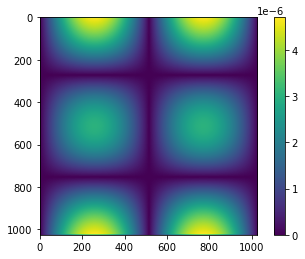
\includegraphics[width=7.5cm]{Images/stokes/Laplace Dirichlet 2D (V)/erreur.png}
    \caption{Champ d'erreurs pour le Laplacien sur $\mathcal{T}^V$}
\end{figure}

\begin{figure}[htp]
    \centering
    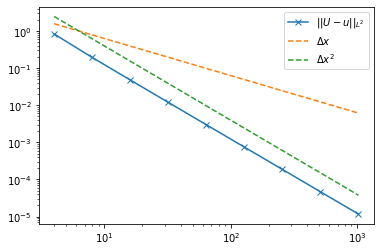
\includegraphics[width=7.5cm]{Images/stokes/Laplace Dirichlet 2D (V)/analyse.png}
    \caption{Analyse de la norme $L^2(\Omega)$ pour le Laplacien sur $\mathcal{T}^V$}
\end{figure}

\newpage

\paragraph{Laplacien de Neumann sur le maillage de pression} Cette fois, le problème distingue les noeuds aux coins des noeuds aux bords, des noeuds à l'intérieur. L'équation à l'intérieur est toujours la même, les noeuds aux bords font intervenir quatre points et les noeuds aux coins trois seulement. On approche les conditions de Neumann par une approximation d'ordre 2 de la dérivée de la grandeur $P$.

\begin{minted}{python}
from matplotlib import pyplot
import numpy
from numpy import cos, pi, sin
from scipy import sparse
from scipy.sparse.linalg import gmres, splu

# SETUP
u_func    = lambda x, y : cos(x) * sin(y)
dudx_func = lambda x, y : -sin(x) * sin(y)
dudy_func = lambda x, y :  cos(x) * cos(y)
Su_func   = lambda x, y : 2 * u_func(x, y)

# DISCRETISATION SPATIALE
## Horizontale
xi = 0.
xf = 2*pi
nx_ = numpy.array([4, 8, 16, 32, 64, 128, 256, 512, 1024])
dx_ = (xf-xi)/nx_

## Verticale
yi = 0.
yf = 2*pi

# INITIALISATION
err = numpy.zeros(nx_.shape)

# ANALYSE DU SCHEMA
for k, nx in enumerate(nx_):
    
    # Discrétisation spatiale
    dx = dx_[k]
    ny = nx
    print("> Maillage {}x{}".format(ny, nx))
    dy = (yf-yi)/ny
    Ox = numpy.linspace(xi, xf, nx+1)
    Oy = numpy.linspace(yi, yf, ny+1)
    X, Y = numpy.meshgrid(Ox, Oy)
    
    # Construction de l'opérateur discret
    n = 5*(ny-1)*(nx-1) + 2*4*(ny-1) + 2*4*(nx-1) + 3 * 3 + 1
    lignes   = numpy.zeros(n)
    colonnes = numpy.zeros(n)
    donnees  = numpy.zeros(n)
    
    b = (dy*dx) * Su_func(X, Y)
    b[0, 0] = u_func(xi, yi)
    
    
    compteur = 0
    for j in range(ny+1):
        for i in range(nx+1):
            
            if i == 0 and j == 0:
                lignes[compteur]   = j * (nx+1) + i
                colonnes[compteur] = j * (nx+1) + i
                donnees[compteur]  = 1
                compteur += 1

            elif i == 0 and j == ny:
                b[j, i] -= 2*dy*dudx_func(xi, yf)
                b[j, i] += 2*dx*dudy_func(xi, yf)
                lignes[compteur : compteur+3] = j * (nx+1) + i
                colonnes[compteur]   = j * (nx+1) + i
                colonnes[compteur+1] = j * (nx+1) + i + 1
                colonnes[compteur+2] = (j-1) * (nx+1) + i
                donnees[compteur]    = 2 * (dy/dx + dx/dy)
                donnees[compteur+1]  = - 2 * dy / dx
                donnees[compteur+2]  = - 2 * dx / dy
                compteur += 3

            elif i == nx and j == 0:
                b[j, i] += 2*dy*dudx_func(xf, yi)
                b[j, i] -= 2*dx*dudy_func(xf, yi)
                lignes[compteur : compteur+3] = j * (nx+1) + i
                colonnes[compteur]   = j * (nx+1) + i
                colonnes[compteur+1] = j * (nx+1) + i - 1
                colonnes[compteur+2] = (j+1) * (nx+1) + i
                donnees[compteur]    = 2 * (dy/dx + dx/dy)
                donnees[compteur+1]  = - 2 * dy / dx
                donnees[compteur+2]  = - 2 * dx / dy
                compteur += 3

            elif i == nx and j == ny:
                b[j, i] += 2*dy*dudx_func(xf, yf)
                b[j, i] += 2*dx*dudy_func(xf, yf)
                lignes[compteur : compteur+3] = j * (nx+1) + i
                colonnes[compteur]   = j * (nx+1) + i
                colonnes[compteur+1] = j * (nx+1) + i - 1
                colonnes[compteur+2] = (j-1) * (nx+1) + i
                donnees[compteur]    = 2 * (dy/dx + dx/dy)
                donnees[compteur+1]  = - 2 * dy / dx
                donnees[compteur+2]  = - 2 * dx / dy
                compteur += 3
            
            elif i == 0 and j > 0 and j < ny:
                b[j, i] -= 2 * dy * dudx_func(xi, Oy[j])
                lignes[compteur : compteur+4] = j * (nx+1) + i
                colonnes[compteur]   = j * (nx+1) + i
                colonnes[compteur+1] = j * (nx+1) + i + 1
                colonnes[compteur+2] = (j-1) * (nx+1) + i
                colonnes[compteur+3] = (j+1) * (nx+1) + i
                donnees[compteur]    = 2 * (dy/dx + dx/dy)
                donnees[compteur+1]  = - 2 * dy/dx
                donnees[compteur+2]  = - dx/dy
                donnees[compteur+3]  = - dx/dy
                compteur += 4

            elif i == nx and j > 0 and j < ny:
                b[j, i] += 2 * dy * dudx_func(xf, Oy[j])
                lignes[compteur : compteur+4] = j * (nx+1) + i
                colonnes[compteur]   = j * (nx+1) + i
                colonnes[compteur+1] = j * (nx+1) + i - 1
                colonnes[compteur+2] = (j-1) * (nx+1) + i
                colonnes[compteur+3] = (j+1) * (nx+1) + i
                donnees[compteur]    = 2 * (dy/dx + dx/dy)
                donnees[compteur+1]  = - 2 * dy/dx
                donnees[compteur+2]  = - dx/dy
                donnees[compteur+3]  = - dx/dy
                compteur += 4

            elif j == 0 and i > 0 and i < nx:
                b[j, i] -= 2 * dx * dudy_func(Ox[i], yi)
                lignes[compteur : compteur+4] = j * (nx+1) + i
                colonnes[compteur]   = j * (nx+1) + i
                colonnes[compteur+1] = j * (nx+1) + i - 1
                colonnes[compteur+2] = j * (nx+1) + i + 1
                colonnes[compteur+3] = (j+1) * (nx+1) + i
                donnees[compteur]    = 2 * (dy/dx + dx/dy)
                donnees[compteur+1]  = - dy/dx
                donnees[compteur+2]  = - dy/dx
                donnees[compteur+3]  = - 2 * dx/dy
                compteur += 4

            elif j == ny and i > 0 and i < nx:
                b[j, i] += 2 * dx * dudy_func(Ox[i], yf)
                lignes[compteur : compteur+4] = j * (nx+1) + i
                colonnes[compteur]   = j * (nx+1) + i
                colonnes[compteur+1] = j * (nx+1) + i - 1
                colonnes[compteur+2] = j * (nx+1) + i + 1
                colonnes[compteur+3] = (j-1) * (nx+1) + i
                donnees[compteur]    = 2 * (dy/dx + dx/dy)
                donnees[compteur+1]  = - dy/dx
                donnees[compteur+2]  = - dy/dx
                donnees[compteur+3]  = - 2 * dx/dy
                compteur += 4

            else:
                lignes[compteur : compteur+5] = j * (nx+1) + i
                colonnes[compteur]   = j * (nx+1) + i
                colonnes[compteur+1] = j * (nx+1) + i - 1
                colonnes[compteur+2] = j * (nx+1) + i + 1
                colonnes[compteur+3] = (j-1) * (nx+1) + i
                colonnes[compteur+4] = (j+1) * (nx+1) + i
                donnees[compteur]    = 2 * (dy/dx + dx/dy)
                donnees[compteur+1]  = -dy/dx
                donnees[compteur+2]  = -dy/dx
                donnees[compteur+3]  = -dx/dy
                donnees[compteur+4]  = -dx/dy
                compteur += 5

    A = sparse.coo_matrix((donnees, (lignes, colonnes)), shape=((ny+1)*(nx+1), (ny+1)*(nx+1))).tocsc()
    Ma = sparse.linalg.LinearOperator(((ny+1)*(nx+1), (ny+1)*(nx+1)), splu(A).solve)
    
    U = gmres(A, b.flatten(), M=Ma)[0].reshape(ny+1, nx+1)
    
    u = u_func(X, Y)
    err[k] = numpy.sqrt(dy*dx) * numpy.linalg.norm(U-u, ord=2)

# FIGURES
pyplot.figure()
pyplot.loglog(nx_, err, 'x-', label=r"$||U-u||_{L^2}$")
pyplot.loglog(nx_, dx_, '--', label=r"$\Delta x$")
pyplot.loglog(nx_, dx_**2, '--', label=r"$\Delta x^2$")
pyplot.legend()
pyplot.show()

pyplot.figure()
pyplot.imshow(numpy.abs(U-u))
pyplot.colorbar()
pyplot.show()
\end{minted}

\begin{figure}[htp]
    \centering
    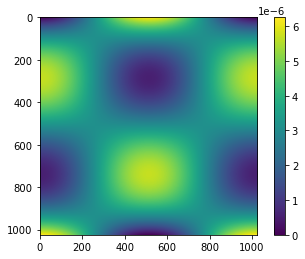
\includegraphics[width=7.5cm]{Images/stokes/Laplace Neumann 2D/erreur.png}
    \caption{Champ d'erreur pour le Laplacien de Neumann, Dirichlet imposé en $(0,0)$ (haut à gauche de l'image)}
\end{figure}

\begin{figure}[htp]
    \centering
    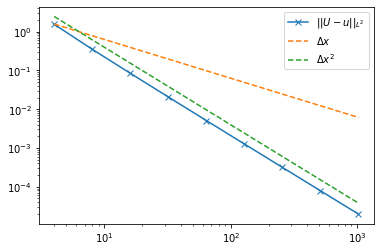
\includegraphics[width=7.5cm]{Images/stokes/Laplace Neumann 2D/analyse.png}
    \caption{Analyse pour le Laplacien de Neumann avec Dirichlet en un point}
\end{figure}

\paragraph{Discrétisation du système de Stokes} On souhaite discrétiser le système de Stokes stationnaire en 2.D posé dans une cavité $\Omega$ ouverte, connexe, bornée et lipschitzienne. On introduit le maillage M.A.C $\mathcal{T}$. On suppose que $\mu = 1.$. Soit le système de Stokes
\begin{align*}
    \partial_x u + \partial_y v = & 0 \\
    -\Delta u + \partial_x p = & f^u \\
    -\Delta v + \partial_y p = & f^v
\end{align*}

La discrétisation en volumes finis de ce système s'effectue en intégrant chaque équation respectivement sur les volumes d'aire $\Delta y \Delta x$ centrés sur des points différents. L'équation de continuité s'intègre sur un volume centré en un point de pression, l'équation de conservation du moment horizontal s'intègre sur un volume centré en $U_{j,i}$ et la conservation du moment vertical s'intègre sur un volume centré en $V_{j,i}$.

Après intégrations par parties et approximation des flux par différences finies d'ordre 1, on trouve pour chaque noeud à l'intérieur :
\begin{align*}
    \frac{\Delta y}{\Delta x} \left( U_{j,i+1} - U_{j,i} \right) + \frac{\Delta x}{\Delta y} \left( V_{j+1,i} - V_{j,i} \right) = 0 \\
    -\frac{\Delta y}{\Delta x} \left( U_{j,i+1} + U_{j,i-1} \right) + -\frac{\Delta x}{\Delta y} \left( U_{j+1,i} + U_{j-1,i} \right) + 2\left( \frac{\Delta y}{\Delta x} + \frac{\Delta x}{\Delta y} \right) + \\ \Delta y \left( P_{j,i} - P_{j,i-1} \right) = \Delta y \Delta x f^u_{j,i} \\
    -\frac{\Delta y}{\Delta x} \left( V_{j,i+1} + V_{j,i-1} \right) + -\frac{\Delta x}{\Delta y} \left( V_{j+1,i} + V_{j-1,i} \right) + 2\left( \frac{\Delta y}{\Delta x} + \frac{\Delta x}{\Delta y} \right) + \\ \Delta x \left( P_{j,i} - P_{j-1, i} \right) = \Delta y \Delta x f^v_{j,i}
\end{align*}

Comme on l'a vu pour les laplaciens traités précédemment, il convient pour d'éliminer les noeuds inexistants grâce aux conditions aux limites de Dirichlet en vitesse pour la deuxième et l'avant-dernière colonne pour $U$ et la deuxième et avant-dernière ligne pour $V$. Les points de vitesse sur le bord vérifiant $U_{j,i} = u^D(x_i, y_j)$, $V_{j,i} = v^D(x_j, y_i)$, respectivement sur les sous-maillages $U$ et $V$ - avec des absisses et ordonnées décalées, donc.

\paragraph{Méthode de pénalisation} On assemble les inconnues sous la forme $$ X := \begin{pmatrix} U \\ V \\ P \end{pmatrix} $$ L'assemblage du système $$ A X = B $$ se fait par blocs $$ A = \begin{pmatrix} A_{uu} & A_{uv} & A_{up} \\ A_{vu} & A_{vv} & A_{vp} \\ A_{pu} & A_{pv} & A_{pp} \end{pmatrix} $$ Les variables $U$ et $V$ sont découplées donc $A_{uv}$ et $A_{vu}$ sont des blocs nuls. D'autre part, on a les égalités $A_{pu} = A_{up}^T$ et $A_{pv} = A_{vp}^T$.

Si le bloc $A_{pp}$ est laissé nul comme le suggère le système alors le problème est en fait mal posé. La méthode de pénalisation consiste en le choix d'un réel strictement positif $\epsilon$ et on propose $$ A_{pp} = \epsilon \text{Id}_{(ny+1)(nx+1)} $$

Dans ce cas le système est résoluble, mais on doit corriger la pression : $$ P = \frac{1}{\epsilon} P $$ Il aurait été utile de vérifier le comportement du schéma en fonction des valeurs de $\epsilon$, chose que je n'ai pas pris le temps de faire. Après quelques échecs d'assemblage et de résolution, il fût décidé que je continue pour passer à la suite et que j'essaie de travailler sur les méthodes de projection scalaire.

\section{Le système de Stokes dépendant du temps}

\paragraph{Système de Stokes dépendant du temps} Le problème de Stokes dépendant du temps avec conditions de Dirichlet en vitesse aux bords s'écrit, avec masse volumique et viscosité dynamique constante,
\begin{align*}
    \nabla \cdot \mathbf{v} = 0 & (0,T) \times \Omega \\
    \rho \partial_t \mathbf{v} - \mu \Delta \mathbf{v} + \nabla p = \rho \mathbf{f} & (0,T) \times \Omega \\
    \mathbf{v}(0, \mathbf{x}) = \mathbf{v}^0(\mathbf{x} & \Omega \\
    \mathbf{v}_{|\partial \Omega}(t, \mathbf{x}) = 0 & (0,T) \times \partial \Omega
\end{align*}

\paragraph{Cadre fonctionnel pour Stokes dépendant du temps} On note $$ H^1_{\int = 0}(\Omega) := \{ q \in L^2(\Omega), \int_\Omega q(x) dx = 0 \} $$ l'espace des fonctions $L^2(\Omega)$ de moyenne nulle. On introduit alors l'espace des fonctions test $$ N(\Omega)^d := \{ \mathbf{v} \in \mathcal{C}^{\infty}_c(\Omega)^d, \nabla \cdot \mathbf{v} = 0 \} $$ On note $H$, respectivement $V$ la fermeture de $N$ dans les espaces $L^2(\Omega)^d$ $H^1_0(\Omega)^d$. Ces deux espaces se caractérisent par $$ H = \{ \mathbf{v} \in L^2(\Omega)^d, \nabla \cdot \mathbf{v}, \mathbf{v} \cdot \mathbf{n} = 0 \} $$ où $\mathbf{n}$ est la normale sortante de $\Omega$ et $$ V = \{ \mathbf{v} \in H^1_0(\Omega)^d, \nabla \cdot \mathbf{v} = 0 \} $$
L'espace $V$ est dense dans $H$ et l'injection de $V$ dans $H$ est continue. De plus, $H$ s'identifie à son dual. On propose donc $$ V \hookrightarrow H \equiv H' \hookrightarrow V' $$ l'identification étant faite à l'aide du produit scalaire de $L^2(\Omega)^d$.

\paragraph{Formulation contrainte du problème} Notons $$ a : H^1_{\int = 0} \times H^1_{\int = 0} \rightarrow \mathbb{R} ; \mathbf{u}, \mathbf{v} \mapsto < \nabla \mathbf{u}, \nabla \mathbf{v} > $$ Alors le problème s'écrit, pour tout $\mathbf{f} \in L^2\left( (0, T), H^{-1}(\Omega)^d \right)$ et $u_0 \in H$, trouver $\mathbf{v} \in \mathcal{W}(V, V')$ tel que
\begin{align*}
    <\partial_t \mathbf{v}, \mathbf{w}>_{V', V} + a(\mathbf{v}, \mathbf{w}) = <\mathbf{f}, \mathbf{w}>_{H^{-1}, H^1_0} & p.p (0, T), \forall \mathbf{w} \in V \\
    \mathbf{v}(0) = \mathbf{v}^0
\end{align*}
avec $\mathcal{W}(V, V') := \{ \mathbf{v} : (0, T) \rightarrow V, \mathbf{v} \in L^2((0,T), V), \partial_t \mathbf{v} \in L^2((0,T), V')\}$ Sous cette forme, on peut montrer que, quel que soit $T>0$, il existe une unique solution au problème. On peut s'inspirer de la preuve de l'existence globale des solutions de Leray présentée dans le chapitre 3 du cours d'Anne-Laure DALIBARD, première partie \href{https://ljll.math.upmc.fr/~dalibard/cours/Notes\%20Chapitre\%203\%20-\%20Equations\%20de\%20Navier-Stokes.pdf}{(disponible ici)}, seul le premier lemme est ici concerné.

\paragraph{Une formulation mixte} On introduit une nouvelle forme, linéaire, $b : \mathcal{L}(H^1_0(\Omega)^d \times L^2_0(\Omega) ; \mathbb{R}) ; \mathbf{w}, q \mapsto (-\nabla\cdot \mathbf{w}, q)_{L^2(\Omega)}$ et alors résoudre le problème de Stokes dépendant du temps est équivalent à trouver $\mathbf{v} \in \mathcal{W}(H^1_0(\Omega)^d, H^{-1}(\Omega)^d)$ et $p \in L^2((0,T), L^2_0(\Omega)$ tels que
\begin{align*}
    (\partial_t \mathbf{v}, \mathbf{w})_{L^2} + b(\mathbf{v}, p) + a(\mathbf{v}, \mathbf{w}) = & (\mathbf{f}, \mathbf{w})_{L^2} & \hspace{5pt} p.p (0, T), \forall \mathbf{w} \in H^1_0(\Omega)^d \\
    \nabla \cdot \mathbf{v} q = & 0 & \hspace{5pt} \forall q \in L^2_0(\Omega)
    \mathbf{v}(0) = \mathbf{v}^0
\end{align*}
Quel que soit $T$ strictement positif, il existe une unique solution du problème. 
 
\section{Analyse numérique pour le problème de Stokes dépendant du temps}

\paragraph{Exemple de l'équation de réaction-diffusion avec Dirichlet aux bords} On développe un code adapté à la résolution de
\begin{align*}
    \partial_t u - \Delta u = S_u \\
    u_{|\partial \Omega} = u^D \\
    u(0, \cdot) = u^0
\end{align*}

On se sert de la fonction analytique suivante $$ u(t, x, y) = sin(x) cos(y) e^{-2t} $$. Alors l'équation est satisfaite pour le second membre $S_u \equiv 0$. 

\begin{minted}{python}
from matplotlib import pyplot
import numpy
from numpy import cos, exp, pi, sin
import scipy
from scipy import sparse
from scipy.sparse import linalg

# SETUP
u_func = lambda t, x, y : sin(x) * cos(y) * exp(-2*t)
Su_func = lambda t, x, y : numpy.zeros(x.shape)

# DISCRETISATION TEMPORELLE
ti = 0.
nt = 1000
dt = .001
tf = ti + nt*dt
T  = tf-ti

# DISCRETISATION SPATIALE
## Horizontale
xi = 0.
xf = 2*pi
nx_ = numpy.array([4, 8, 16, 32, 64, 128, 256])
dx_ = (xf-xi)/nx_

## Verticale
yi = 0.
yf = 2*pi

# INITIALISATION
err = numpy.zeros(nx_.shape)

# ITERATION SPATIALE
for k, nx in enumerate(nx_):
    
    # Discrétisation spatiale
    dx = dx_[k]
    Ox = numpy.linspace(xi, xf, nx+1)
    ny = nx
    dy = (yf-yi)/ny
    Oy = numpy.linspace(yi, yf, ny+1)
    X, Y = numpy.meshgrid(Ox, Oy)
    
    # Construction de l'opérateur discret
    n = 5 * (ny*nx) + 2*(ny+1) + 2*(nx+1)
    lignes   = numpy.zeros(n)
    colonnes = numpy.zeros(n)
    donnees  = numpy.zeros(n)
    compteur = 0
    
    for j in range(ny+1):
        for i in range(nx+1):
            
            if i == 0 or i == nx or j == 0 or j == ny:
                lignes[compteur]   = j * (nx+1) + i
                colonnes[compteur] = j * (nx+1) + i
                donnees[compteur]  = 1
                compteur += 1
                
            else:
                lignes[compteur : compteur+5] = j * (nx+1) + i
                colonnes[compteur]   = j * (nx+1) + i
                colonnes[compteur+1] = j * (nx+1) + i + 1
                colonnes[compteur+2] = j * (nx+1) + i - 1
                colonnes[compteur+3] = (j-1) * (nx+1) + i
                colonnes[compteur+4] = (j+1) * (nx+1) + i
                donnees[compteur] = 2 * (dy/dx + dx/dy) + dx*dy/dt
                donnees[compteur+1] = -dy/dx
                donnees[compteur+2] = -dy/dx
                donnees[compteur+3] = -dx/dy
                donnees[compteur+4] = -dx/dy
                compteur += 5
    
    A = sparse.coo_matrix((donnees, (lignes, colonnes)), shape=((ny+1)*(nx+1), (ny+1)*(nx+1))).tocsc()
    Ma = linalg.LinearOperator(((ny+1)*(nx+1), (ny+1)*(nx+1)), linalg.splu(A).solve)
    
    # Initialisation
    U = u_func(0, X, Y)
    
    # Itération temporelle
    for n in range(nt+1):
        # info
        if n%10 == 0: print("> grille {}x{}, itération {}/{}".format(ny, nx, n, nt))
        
        # date courante
        t = ti + (n+1)*dt
        
        # construction du second membre
        b = dy*dx * Su_func(t, X, Y) + dy*dx/dt * U
        b[0, :] = u_func(t, Ox, yi)
        b[-1,:] = u_func(t, Oy, yf)
        b[:, 0] = u_func(t, xi, Oy)
        b[:,-1] = u_func(t, xf, Oy)
        
        # Résolution
        U = linalg.gmres(A, b.flatten(), M=Ma)[0].reshape((ny+1, nx+1))
        
    u = u_func(tf, X, Y)    
    err[k] = numpy.sqrt(dy*dx) * numpy.linalg.norm(U-u, ord=2)

# FIGURES
pyplot.suptitle(r"$\epsilon := ||U_h(t_f, \cdot, \cdot) - u_h(t_f, \cdot, \cdot)||$ ; $\Delta t$={}, $N_t$={}".format(dt, nt))
pyplot.loglog(nx_, err, 'x-', label="$\ln(\epsilon)$")
pyplot.loglog(nx_, dx_, label="$\Delta x$")
pyplot.loglog(nx_, dx_**2, label="$\Delta x^2$")
pyplot.legend()
pyplot.xlabel(r"$N_x$")
pyplot.show()

pyplot.figure()
pyplot.imshow(numpy.abs(U-u))
pyplot.colorbar()
pyplot.show()
\end{minted}
On fait tourner la simulation sur trois couples $(\Delta t, n_t)$.

\begin{figure}[htp]
    \centering
    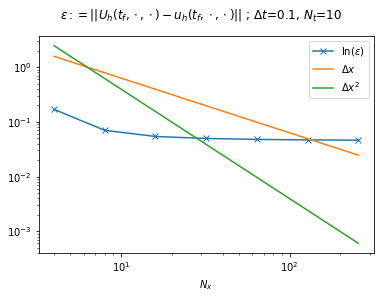
\includegraphics[width=7.5cm]{Images/stokes/Parbolique 2D/analyse 1.png}
    \caption{}
\end{figure}

\begin{figure}[htp]
    \centering
    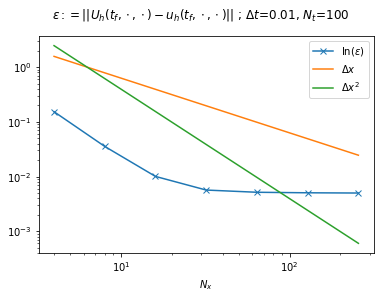
\includegraphics[width=7.5cm]{Images/stokes/Parbolique 2D/analyse 2.png}
    \caption{}
\end{figure}

\begin{figure}[htp]
    \centering
    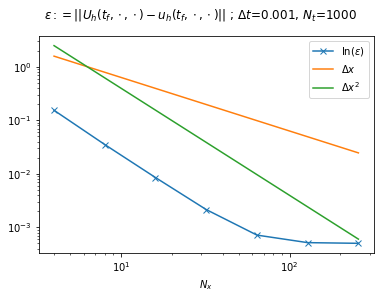
\includegraphics[width=7.5cm]{Images/stokes/Parbolique 2D/analyse 3.png}
    \caption{}
\end{figure}

\begin{figure}[htp]
    \centering
    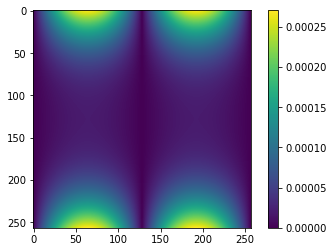
\includegraphics[width=7.5cm]{Images/stokes/Parbolique 2D/erreur 3.png}
    \caption{Champ d'erreur au temps final pour $\Delta t = 10^{-3}$}
\end{figure}

On trouve bien que l'erreur rencontre un plancher autour de $\Delta t$, c'est la conséquence du premier ordre en temps du schéma d'Euler implicite. D'autres méthodes peuvent être employées, les méthodes explicites imposant une condition de Courant–Friedrichs–Lewy pour assurer leur stabilité. Dans ce genre de méthode, on prescrit cette condition et on calcule $\Delta t$ en fonction de $\Delta x$ et de la C.F.L. Une bonne pratiqe est d'implémenter la discrétisation spatiale en premier lieu.

\paragraph{Une méthode de projection} Les méthodes de projections pour les fluides incompressibles ont été synthétisées dans l'article \cite{guermond}, section 3.1. Leur intérêt réside dans l'obtention d'une suite d'équations elliptiques indépendantes, là où les variables vitesses et pression sont couplées dans le système de Stokes.

La décomposition de Helmholtz de l'espace $L^2(\Omega)^d$ s'écrit avec $$ H := \{ \mathbf{v} \in L^2(\Omega)^d, \nabla \cdot \mathbf{v} = 0, \mathbf{v} \cdot \mathbf{n}_{|\partial \Omega} = 0 \} $$ et $$ G := \{ \mathbf{v} \in L^2(\Omega)^d, \mathbf{v} = \nabla \phi, \phi \in H^1(\Omega)/\mathbb{R} \} $$
Pour chaque $\mathbf{v}$, il existe un unique couple $\mathbf{v}_{\phi}, \mathbf{v}_{\psi}$ tel que $\mathbf{v} = \mathbf{v}_{\phi} + \mathbf{v}_\psi$ et les vecteurs du membre de droite sont orthogonaux.

Dans la décomposition précédente, $\mathbf{v}_\phi = \nabla \phi \in G$ et $\mathbf{v}_\psi = \nabla \times \psi \in H$. Le domaine étant connexe, il est simplement connexe et donc $\nabla \psi = 0$.

Pour un potentiel scalaire $\phi$, on a le problème de Poisson donné avec conditions de Neumann au bord
\begin{align*}
    \Delta \phi = & \nabla \mathbf{v} \\
    \nabla \phi \cdot \mathbf{n}_{|\partial \Omega} = & \mathbf{v} \cdot \mathbf{n}_{|\partial \Omega}
\end{align*}
et alors $\mathbf{v}_\phi = \nabla \phi$ et $\mathbf{v}_\psi := \mathbf{v} - \mathbf{v} - \nabla \phi$

L'algotithme commence par un étape de prédiction, on résoud
\begin{align*}
    \frac{\tilde{\mathbf{v}} - \mathbf{v}^{(n)}}{\Delta t} - \mu \Delta \tilde{\mathbf{v}}^{(n+1)} + \nabla p^{(n)} = & \mathbf{f}^{(n+1)} \\
    \tilde{\mathbf{v}}^{(n+1)} = & \mathbf{v}^D
\end{align*}

L'algorithme se poursuit par l'étape de projection, on résoud cette fois
\begin{align*}
    \nabla \cdot \nabla \phi^{(n+1)} = & \nabla \cdot \tilde{\mathbf{v}}^{(n+1)} \\
    \nabla \phi^{(n+1)} \cdot \mathbf{n}_{|\partial \Omega} = & 0
\end{align*}

et il se termine par la correction de la vitesse, on calcule
\begin{align*}
    \mathbf{v}^{(n+1)} = \tilde{\mathbf{v}}^{(n+1)} - \Delta t \nabla \phi^{(n+1)} \\
    \Phi^{(n+1)} = P^{(n+1)} - P^{(n)}
\end{align*}

On dispose du théorème

\begin{theoreme}
    Soit $(\mathbf{v}, p)$ une solution du problème de Stokes dépendant du temps, et lisse. Alors la solution $(\mathbf{v}_h, p_h)$ de l'algorithme proposé vérifie
    \begin{align*}
        \| \mathbf{v}_{\Delta t} - \mathbf{v}_{h, \Delta t} \|_{l^{\infty}(L^2(\Omega)} + \| \mathbf{v}_{\Delta t} - \tilde{\mathbf{v}}_{h, \Delta t} & \leqslant c(\mathbf{u}, p, T) \Delta t \\
        \| p_{\Delta t} - p_{h, \Delta t} \|_{l^{\infty}(L^2(\Omega)} + \| \mathbf{v}_{\Delta t} - \tilde{\mathbf{v}}_{h, \Delta t} \|_{l^{\infty}(H^1(\Omega)} & \leqslant c(\mathbf{v}, p, T) \sqrt{\Delta t}
    \end{align*}
\end{theoreme}

\paragraph{Implémentation de projection scalaire pour Stokes 2.D} On étudie l'évolution d'un tourbillon de Taylor-Green initialisé à $t=0$.

\begin{minted}{python}
from matplotlib import pyplot
import numpy
from numpy import cos, exp, pi, sin
from scipy import sparse
from scipy.sparse.linalg import gmres, splu

# PHASE LIQUIDE
rho = 1.
mu  = 1.

# SETUP
u_func  = lambda t, x, y :  sin(x)*cos(y)*exp(-2*t)
v_func  = lambda t, x, y : -cos(x)*sin(y)*exp(-2*t)
p_func  = lambda t, x, y :  numpy.zeros(x.shape)
dudx_func = lambda t, x, y :  cos(x)*cos(y)*exp(-2*t)
dvdy_func = lambda t, x, y : -cos(x)*cos(y)*exp(-2*t)
dpdx_func = lambda t, x, y :  numpy.zeros(x.shape)
dpdy_func = lambda t, x, y :  numpy.zeros(x.shape)
Su_func = lambda t, x, y :  numpy.zeros(x.shape)
Sv_func = lambda t, x, y :  numpy.zeros(x.shape)

# DISCRETISATION TEMPORELLE
ti = 0.
nt = 1000
dt = .001
tf = ti + nt*dt

# DISCRETISATION SPATIALE
xi  = 0.
xf  = 2*pi
nx_ = numpy.array([4, 8, 16, 32, 64, 128, 256])
dx_ = numpy.zeros(nx_.shape)

# INITIALISATION
## err[k, 0] : erreur sur la variable U pour nx_[k]**2 volumes
## err[k, 1] : erreur sur la variable V pour nx_[k]**2 volumes
## err[k, 2] : erreur sur la variable P pour nx_[k]**2 volumes
## err[k, 3] : erreur sur la variable D pour nx_[k]**2 volumes ; D pour div 
err = numpy.zeros((nx_.shape[0], 4))

# ANALYSE
for k, nx in enumerate(nx_):
    
    # Discrétisation spatiale
    ## horizontale
    dx = (xf-xi)/nx
    dx_[k] = dx
    x_c = numpy.concatenate([[xi], numpy.linspace(xi+dx/2, xf-dx/2, nx), [xf]], axis=0)
    x_f = numpy.linspace(xi, xf, nx+1)
    ## verticale
    yi = xi
    yf = xf
    ny = nx
    dy = (yf-yi)/ny
    y_c = numpy.concatenate([[yi], numpy.linspace(yi+dx/2, yf-dx/2, ny), [yf]], axis=0)
    y_f = numpy.linspace(yi, yf, ny+1)
    ## 2.D
    Xu, Yu = numpy.meshgrid(x_c, y_f)
    Xv, Yv = numpy.meshgrid(x_f, y_c)
    Xp, Yp = numpy.meshgrid(x_f, y_f)
    
    # Initialisation
    U = u_func(ti, Xu, Yu)
    V = v_func(ti, Xv, Yv)
    P = numpy.zeros(Xp.shape)
    ## construction de la divergence initiale
    D = (U[:,1:]-U[:,:-1])/dx + (V[1:,:]-V[:-1,:])/dy
    D[0, 1:-1]  = (U[0,2:-1]-U[0,1:-2])/dx + 2/dy*(V[1,1:-1]-V[0,1:-1])
    D[-1, 1:-1] = (U[-1,2:-1]-U[-1,1:-2])/dx + 2/dy*(V[-1,1:-1]-V[-2,1:-1])
    D[1:-1, 0]  = 2/dx*(U[1:-1,1]-U[1:-1,0]) + (V[2:-1,0]-V[1:-2,0])/dy
    D[1:-1,-1]  = 2/dx*(U[1:-1,-1]-U[1:-1,-2]) + (V[2:-1,-1]-V[1:-2,-1])/dy
    D[0, 0]  = 2/dx*(U[0,1]-U[0,0]) + 2/dy*(V[1,0]-V[0,0])
    D[-1, 0] = 2/dx*(U[0,1]-U[0,0]) + 2/dy*(V[-1,0]-V[-2,0])
    D[-1,-1] = 2/dx*(U[0,-1]-U[0,-2]) + 2/dy*(V[-1,0]-V[-2,0])
    D[0,-1]  = 2/dx*(U[0,-1]-U[0,-2]) + 2/dy*(V[1,0]-V[0,0])

    if nx == nx_[-1]:
        ## contrôle de la U initiale
        pyplot.imshow(U)
        pyplot.colorbar()
        pyplot.suptitle(r"$U({}, \cdot, \cdot)$ ; {}x{} vol ; $n_t$={}, $\Delta t$={}".format(ti, ny, nx, nt, dt))
        pyplot.show()
        ## contrôle de la vitesse V initiale
        pyplot.imshow(V)
        pyplot.colorbar()
        pyplot.suptitle(r"$V({}, \cdot, \cdot)$ ; {}x{} vol ; $n_t$={}, $\Delta t$={}".format(ti, ny, nx, nt, dt))
        pyplot.show()
        ## contrôle de la divergence initiale
        pyplot.imshow(P)
        pyplot.colorbar()
        pyplot.suptitle(r"$P({}, \cdot, \cdot)$ ; {}x{} vol ; $n_t$={}, $\Delta t$={}".format(ti, ny, nx, nt, dt))
        pyplot.show()
        ## contrôle de la divergence initiale
        pyplot.imshow(numpy.abs(D))
        pyplot.colorbar()
        pyplot.suptitle(r"$|div(u, v)({}, \cdot, \cdot)|$ ; {}x{} vol ; $n_t$={}, $\Delta t$={}".format(ti, ny, nx, nt, dt))
        pyplot.show()
    
    # Construction des opérateurs creux
    ## prédicteur de la vitesse U
    N = 5*(ny-1)*nx + 2*(ny-1) + 2*(nx+2)
    lignes   = numpy.zeros(N)
    colonnes = numpy.zeros(N)
    donnees  = numpy.zeros(N)

    compteur = 0
    for j in range(ny+1):
        for i in range(nx+2):
                
            if i == 0 or i == nx+1 or j == 0 or j == ny:
                lignes[compteur]   = j * (nx+2) + i
                colonnes[compteur] = j * (nx+2) + i
                donnees[compteur]  = 1
                compteur += 1
   
            elif i == 1:
                lignes[compteur : compteur+5] = j * (nx+2) + i
                colonnes[compteur]   = j * (nx+2) + i
                colonnes[compteur+1] = j * (nx+2) + i - 1
                colonnes[compteur+2] = j * (nx+2) + i + 1
                colonnes[compteur+3] = (j-1) * (nx+2) + i
                colonnes[compteur+4] = (j+1) * (nx+2) + i
                donnees[compteur]    = 3*(dy/dx) + 2*(dx/dy) + (dy*dx)/dt
                donnees[compteur+1]  = -2*dy/dx
                donnees[compteur+2]  = -dy/dx
                donnees[compteur+3]  = -dx/dy
                donnees[compteur+4]  = -dx/dy
                compteur += 5
            
            elif i == nx:
                lignes[compteur : compteur+5] = j * (nx+2) + i
                colonnes[compteur]   = j * (nx+2) + i
                colonnes[compteur+1] = j * (nx+2) + i - 1
                colonnes[compteur+2] = j * (nx+2) + i + 1
                colonnes[compteur+3] = (j-1) * (nx+2) + i
                colonnes[compteur+4] = (j+1) * (nx+2) + i
                donnees[compteur]    = 3*(dy/dx) + 2*(dx/dy) + (dy*dx)/dt
                donnees[compteur+1]  = -dy/dx
                donnees[compteur+2]  = -2*dy/dx
                donnees[compteur+3]  = -dx/dy
                donnees[compteur+4]  = -dx/dy
                compteur += 5

            else:
                lignes[compteur : compteur+5] = j * (nx+2) + i
                colonnes[compteur]   = j * (nx+2) + i
                colonnes[compteur+1] = j * (nx+2) + i - 1
                colonnes[compteur+2] = j * (nx+2) + i + 1
                colonnes[compteur+3] = (j-1) * (nx+2) + i
                colonnes[compteur+4] = (j+1) * (nx+2) + i
                donnees[compteur]    = 2 * (dy/dx + dx/dy) + (dy*dx)/dt
                donnees[compteur+1]  = -dy/dx
                donnees[compteur+2]  = -dy/dx
                donnees[compteur+3]  = -dx/dy
                donnees[compteur+4]  = -dx/dy
                compteur += 5

    Auu = sparse.coo_matrix((donnees, (lignes, colonnes)), shape=((ny+1)*(nx+2), (ny+1)*(nx+2))).tocsc()
    Mau = sparse.linalg.LinearOperator(((ny+1)*(nx+2), (ny+1)*(nx+2)), splu(Auu).solve)
    
    # Construction des opérateurs creux et des seconds membres
    ## prédicteur de la vitesse V
    N = 5*ny*(nx-1) + 2*(ny+2) + 2*(nx-1)
    lignes   = numpy.zeros(N)
    colonnes = numpy.zeros(N)
    donnees  = numpy.zeros(N)
    
    compteur = 0
    for j in range(ny+2):
        for i in range(nx+1):
                
            if i == 0 or i == nx or j == 0 or j == ny+1:
                lignes[compteur]   = j * (nx+1) + i
                colonnes[compteur] = j * (nx+1) + i
                donnees[compteur]  = 1
                compteur += 1
   
            elif j == 1:
                lignes[compteur : compteur+5] = j * (nx+1) + i
                colonnes[compteur]   = j * (nx+1) + i
                colonnes[compteur+1] = j * (nx+1) + i - 1
                colonnes[compteur+2] = j * (nx+1) + i + 1
                colonnes[compteur+3] = (j-1) * (nx+1) + i
                colonnes[compteur+4] = (j+1) * (nx+1) + i
                donnees[compteur]    = 2*(dy/dx) + 3*(dx/dy) + (dy*dx)/dt
                donnees[compteur+1]  = -dy/dx
                donnees[compteur+2]  = -dy/dx
                donnees[compteur+3]  = -2 * dx/dy
                donnees[compteur+4]  = -dx/dy
                compteur += 5
            
            elif j == ny:
                lignes[compteur : compteur+5] = j * (nx+1) + i
                colonnes[compteur]   = j * (nx+1) + i
                colonnes[compteur+1] = j * (nx+1) + i - 1
                colonnes[compteur+2] = j * (nx+1) + i + 1
                colonnes[compteur+3] = (j-1) * (nx+1) + i
                colonnes[compteur+4] = (j+1) * (nx+1) + i
                donnees[compteur]    = 2*(dy/dx) + 3*(dx/dy) + (dy*dx)/dt
                donnees[compteur+1]  = -dy/dx
                donnees[compteur+2]  = -dy/dx
                donnees[compteur+3]  = -dx/dy
                donnees[compteur+4]  = -2 * dx/dy
                compteur += 5

            else:
                lignes[compteur : compteur+5] = j * (nx+1) + i
                colonnes[compteur]   = j * (nx+1) + i
                colonnes[compteur+1] = j * (nx+1) + i - 1
                colonnes[compteur+2] = j * (nx+1) + i + 1
                colonnes[compteur+3] = (j-1) * (nx+1) + i
                colonnes[compteur+4] = (j+1) * (nx+1) + i
                donnees[compteur]    = 2 * (dy/dx + dx/dy) + (dy*dx)/dt
                donnees[compteur+1]  = -dy/dx
                donnees[compteur+2]  = -dy/dx
                donnees[compteur+3]  = -dx/dy
                donnees[compteur+4]  = -dx/dy
                compteur += 5

    Avv = sparse.coo_matrix((donnees, (lignes, colonnes)), shape=((ny+2)*(nx+1), (ny+2)*(nx+1))).tocsc()
    Mav = sparse.linalg.LinearOperator(((ny+2)*(nx+1), (ny+2)*(nx+1)), splu(Avv).solve)
    
    # Construction des opérateurs creux
    ## Poisson pour la pression
    N = 5*(ny-1)*(nx-1) + 2*4*(ny-1) + 2*4*(nx-1) + 3 * 3 + 1
    lignes   = numpy.zeros(N)
    colonnes = numpy.zeros(N)
    donnees  = numpy.zeros(N)

    compteur = 0
    for j in range(ny+1):
        for i in range(nx+1):
            
            if i == 0 and j == 0:
                lignes[compteur]   = j * (nx+1) + i
                colonnes[compteur] = j * (nx+1) + i
                donnees[compteur]  = 1
                compteur += 1

            elif i == 0 and j == ny:
                lignes[compteur : compteur+3] = j * (nx+1) + i
                colonnes[compteur]   = j * (nx+1) + i
                colonnes[compteur+1] = j * (nx+1) + i + 1
                colonnes[compteur+2] = (j-1) * (nx+1) + i
                donnees[compteur]    = - 2 * (dy/dx + dx/dy)
                donnees[compteur+1]  = 2 * dy / dx
                donnees[compteur+2]  = 2 * dx / dy
                compteur += 3

            elif i == nx and j == 0:
                lignes[compteur : compteur+3] = j * (nx+1) + i
                colonnes[compteur]   = j * (nx+1) + i
                colonnes[compteur+1] = j * (nx+1) + i - 1
                colonnes[compteur+2] = (j+1) * (nx+1) + i
                donnees[compteur]    = - 2 * (dy/dx + dx/dy)
                donnees[compteur+1]  = 2 * dy / dx
                donnees[compteur+2]  = 2 * dx / dy
                compteur += 3

            elif i == nx and j == ny:
                lignes[compteur : compteur+3] = j * (nx+1) + i
                colonnes[compteur]   = j * (nx+1) + i
                colonnes[compteur+1] = j * (nx+1) + i - 1
                colonnes[compteur+2] = (j-1) * (nx+1) + i
                donnees[compteur]    = - 2 * (dy/dx + dx/dy)
                donnees[compteur+1]  = 2 * dy / dx
                donnees[compteur+2]  = 2 * dx / dy
                compteur += 3
            
            elif i == 0 and j > 0 and j < ny:
                lignes[compteur : compteur+4] = j * (nx+1) + i
                colonnes[compteur]   = j * (nx+1) + i
                colonnes[compteur+1] = j * (nx+1) + i + 1
                colonnes[compteur+2] = (j-1) * (nx+1) + i
                colonnes[compteur+3] = (j+1) * (nx+1) + i
                donnees[compteur]    = - 2 * (dy/dx + dx/dy)
                donnees[compteur+1]  = 2 * dy/dx
                donnees[compteur+2]  = dx/dy
                donnees[compteur+3]  = dx/dy
                compteur += 4

            elif i == nx and j > 0 and j < ny:
                lignes[compteur : compteur+4] = j * (nx+1) + i
                colonnes[compteur]   = j * (nx+1) + i
                colonnes[compteur+1] = j * (nx+1) + i - 1
                colonnes[compteur+2] = (j-1) * (nx+1) + i
                colonnes[compteur+3] = (j+1) * (nx+1) + i
                donnees[compteur]    = - 2 * (dy/dx + dx/dy)
                donnees[compteur+1]  = 2 * dy/dx
                donnees[compteur+2]  = dx/dy
                donnees[compteur+3]  = dx/dy
                compteur += 4

            elif j == 0 and i > 0 and i < nx:
                lignes[compteur : compteur+4] = j * (nx+1) + i
                colonnes[compteur]   = j * (nx+1) + i
                colonnes[compteur+1] = j * (nx+1) + i - 1
                colonnes[compteur+2] = j * (nx+1) + i + 1
                colonnes[compteur+3] = (j+1) * (nx+1) + i
                donnees[compteur]    = - 2 * (dy/dx + dx/dy)
                donnees[compteur+1]  = dy/dx
                donnees[compteur+2]  = dy/dx
                donnees[compteur+3]  = 2 * dx/dy
                compteur += 4

            elif j == ny and i > 0 and i < nx:
                lignes[compteur : compteur+4] = j * (nx+1) + i
                colonnes[compteur]   = j * (nx+1) + i
                colonnes[compteur+1] = j * (nx+1) + i - 1
                colonnes[compteur+2] = j * (nx+1) + i + 1
                colonnes[compteur+3] = (j-1) * (nx+1) + i
                donnees[compteur]    = - 2 * (dy/dx + dx/dy)
                donnees[compteur+1]  = dy/dx
                donnees[compteur+2]  = dy/dx
                donnees[compteur+3]  = 2 * dx/dy
                compteur += 4

            else:
                lignes[compteur : compteur+5] = j * (nx+1) + i
                colonnes[compteur]   = j * (nx+1) + i
                colonnes[compteur+1] = j * (nx+1) + i - 1
                colonnes[compteur+2] = j * (nx+1) + i + 1
                colonnes[compteur+3] = (j-1) * (nx+1) + i
                colonnes[compteur+4] = (j+1) * (nx+1) + i
                donnees[compteur]    = - 2 * (dy/dx + dx/dy)
                donnees[compteur+1]  = dy/dx
                donnees[compteur+2]  = dy/dx
                donnees[compteur+3]  = dx/dy
                donnees[compteur+4]  = dx/dy
                compteur += 5
    
    App = sparse.coo_matrix((donnees, (lignes, colonnes)), shape=((ny+1)*(nx+1), (ny+1)*(nx+1))).tocsc()
    Map = sparse.linalg.LinearOperator(((ny+1)*(nx+1), (ny+1)*(nx+1)), splu(App).solve)
    
    # Itération temporelle
    for n in range(nt):
        
        # Info
        if n % 10 == 0: print("> {}x{} volumes, itération {}/{}".format(ny, nx, n, nt))
        
        # Date
        t = ti + (n+1)*dt
        
        # Prédiction de la vitesse U
        ## second membre
        bu = (dx*dy) * Su_func(t, Xu, Yu) + (dx*dy)/dt * U
        bu[0, :] = u_func(t, x_c, yi)
        bu[-1,:] = u_func(t, x_c, yf)
        bu[:, 0] = u_func(t, xi, y_f)
        bu[:,-1] = u_func(t, xf, y_f)
        
        ## résolution
        U = gmres(Auu, bu.flatten(), M=Mau)[0].reshape((ny+1, nx+2))
        
        # Prédiction de la vitesse V
        ## second membre
        bv = (dx*dy) * Sv_func(t, Xv, Yv) + (dx*dy)/dt * V
        bv[0, :] = v_func(t, x_f, yi)
        bv[-1,:] = v_func(t, x_f, yf)
        bv[:, 0] = v_func(t, xi, y_c)
        bv[:,-1] = v_func(t, xf, y_c)
        
        ## résolution
        V = gmres(Avv, bv.flatten(), M=Mav)[0].reshape((ny+2, nx+1))
        
        # Construction de la divergence
        D = (U[:,1:]-U[:,:-1])/dx + (V[1:,:]-V[:-1,:])/dy
        D[0, 1:-1]  = (U[0,2:-1]-U[0,1:-2])/dx + 2/dy*(V[1,1:-1]-V[0,1:-1])
        D[-1, 1:-1] = (U[-1,2:-1]-U[-1,1:-2])/dx + 2/dy*(V[-1,1:-1]-V[-2,1:-1])
        D[1:-1, 0]  = 2/dx*(U[1:-1,1]-U[1:-1,0]) + (V[2:-1,0]-V[1:-2,0])/dy
        D[1:-1,-1]  = 2/dx*(U[1:-1,-1]-U[1:-1,-2]) + (V[2:-1,-1]-V[1:-2,-1])/dy
        D[0, 0]  = 2/dx*(U[0,1]-U[0,0]) + 2/dy*(V[1,0]-V[0,0])
        D[-1, 0] = 2/dx*(U[0,1]-U[0,0]) + 2/dy*(V[-1,0]-V[-2,0])
        D[-1,-1] = 2/dx*(U[0,-1]-U[0,-2]) + 2/dy*(V[-1,0]-V[-2,0])
        D[0,-1]  = 2/dx*(U[0,-1]-U[0,-2]) + 2/dy*(V[1,0]-V[0,0])
        
        # Projection, résolution de Phi
        Phi = gmres(App, (dx*dy)*D.flatten(), M=Map)[0].reshape((ny+1, nx+1))
        
        # Correction des vitesses U, V et de la pression P
        U[1:-1, 1:-1] = U[1:-1, 1:-1] - dt * (Phi[1:-1, 1:]-Phi[1:-1, :-1])/dx
        V[1:-1, 1:-1] = V[1:-1, 1:-1] - dt * (Phi[1:, 1:-1]-Phi[:-1, 1:-1])/dy
        P = P + dt * Phi
    
    # Solution analytiques
    u = u_func(t, Xu, Yu)
    v = v_func(t, Xv, Yv)
    p = p_func(t, Xp, Yp)
    d = dudx_func(t, Xp, Yp) + dvdy_func(t, Xp, Yp)
    
    # Calcul des erreurs
    err[k, 0] = numpy.sqrt(dy*dx) * numpy.linalg.norm(U-u, ord=2)
    err[k, 1] = numpy.sqrt(dy*dx) * numpy.linalg.norm(V-v, ord=2)
    err[k, 2] = numpy.sqrt(dy*dx) * numpy.linalg.norm(P-p, ord=2)
    err[k, 3] = numpy.sqrt(dy*dx) * numpy.linalg.norm(D-d, ord=2)

    # Champs d'erreur
    if nx == nx_[-1]:
        ## Champs d'erreur par variable
        pyplot.imshow(numpy.abs(U-u))
        pyplot.colorbar()
        pyplot.suptitle(r"$U({}, \cdot, \cdot)$ ; {}x{} vol ; $n_t$={}, $\Delta t$={}".format(t, ny, nx, nt, dt))
        pyplot.show()
        
        pyplot.imshow(numpy.abs(V-v))
        pyplot.colorbar()
        pyplot.suptitle(r"$V({}, \cdot, \cdot)$ ; {}x{} vol ; $n_t$={}, $\Delta t$={}".format(t, ny, nx, nt, dt))
        pyplot.show()
        
        pyplot.imshow(numpy.abs(P-p))
        pyplot.colorbar()
        pyplot.suptitle(r"$P({}, \cdot, \cdot)$ ; {}x{} vol ; $n_t$={}, $\Delta t$={}".format(t, ny, nx, nt, dt))
        pyplot.show()    
        
        pyplot.imshow(numpy.abs(D))
        pyplot.colorbar()
        pyplot.suptitle(r"$|div(u, v)({}, \cdot, \cdot)|$ ; {}x{} vol ; $n_t$={}, $\Delta t$={}".format(t, ny, nx, nt, dt))
        pyplot.show()

# ANALYSE
pyplot.figure()
pyplot.loglog(nx_, err[:, 0], 'x-', label=r"$ln(\epsilon_u)$")
pyplot.loglog(nx_, err[:, 1], 'x-', label=r"$ln(\epsilon_v)$")
pyplot.loglog(nx_, err[:, 2], 'x-', label=r"$ln(\epsilon_p)$")
pyplot.loglog(nx_, err[:, 3], 'x-', label=r"$ln(\epsilon_d)$")
pyplot.loglog(nx_, dx_, '--', label=r"$\Delta x$")
pyplot.loglog(nx_, dx_**2, '--', label=r"$\Delta x^2$")
pyplot.legend()
pyplot.suptitle(r"$\epsilon_X := || X({}, \cdot, \cdot) - x({}, \cdot, \cdot) ||$ ; dt={}, $n_t$={}".format(t, t, dt, nt))
pyplot.xlabel(r"$ln(N_x)$")
pyplot.show()
\end{minted}

\begin{figure}[htp]
    \centering
    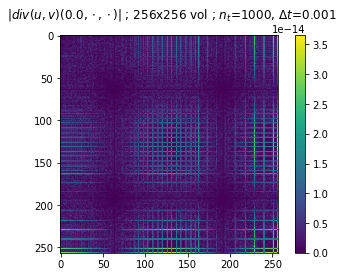
\includegraphics[width=7.5cm]{Images/stokes/sip/Dh0.png}
    \caption{Validation de la méthode de reconstruction de la divergence sur les points de pression à partir des vitesses initiales}
\end{figure}

\begin{figure}[htp]
    \centering
    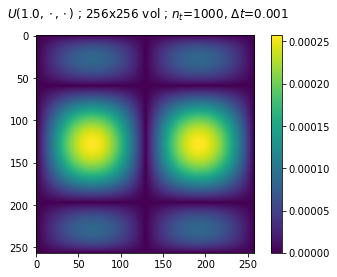
\includegraphics[width=7.5cm]{Images/stokes/sip/Uh.png}
    \caption{Champ d'erreur de $U_h$ au temps final}
\end{figure}

\begin{figure}[htp]
    \centering
    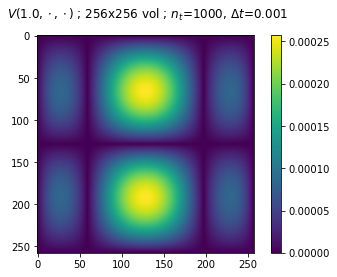
\includegraphics[width=7.5cm]{Images/stokes/sip/Vh.png}
    \caption{Champ d'erreur de $V_h$ au temps final}
\end{figure}

\begin{figure}[htp]
    \centering
    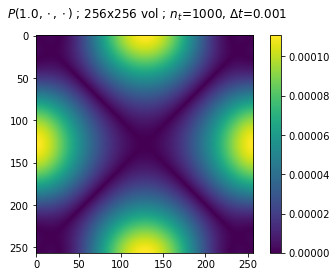
\includegraphics[width=7.5cm]{Images/stokes/sip/Ph.png}
    \caption{Champ d'erreur de la pression au temps final}
\end{figure}

\begin{figure}[htp]
    \centering
    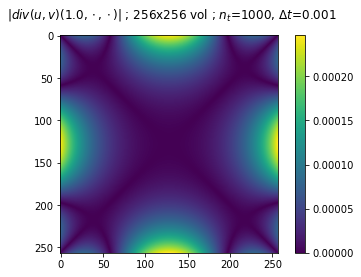
\includegraphics[width=7.5cm]{Images/stokes/sip/Dh.png}
    \caption{Champ d'erreur de la divergence au temps final}
\end{figure}

\begin{figure}[htp]
    \centering
    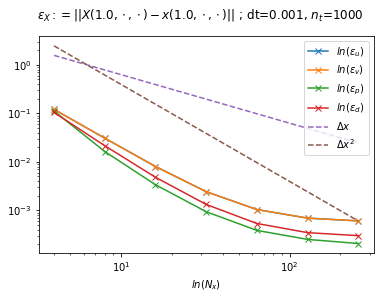
\includegraphics[width=7.5cm]{Images/stokes/sip/analyse.png}
    \caption{Analyse de la méthode S.I.P pour Stokes. Les deux courbes de vitesses sont confondues}
\end{figure}

\newpage

\section{Conclusion}

Ce chapitre a été l'occasion de présenter les concepts de la mécanique des fluides, et ses méthodes d'analyse pour le problème de Stokes. On a un très bref aperçu de la variétés de méthodes existantes pour traiter numériquement des questions d'écoulement visqueux. Après avoir étudié le caractère bien posé des équations, on a introduit un maillage décalé et discrétisé ce problème en volumes finis avant de se pencher sur les algorithmes permettant d'approcher une solution classique en deux dimensions du problème continu. Si ce chapitre occupe beaucoup de place dans le mémoire, il a exigé plus de temps encore durant mon stage. 